\chapter{Road Network Propeties}
\label{ch:properties}

\todo[inline]{Add a short introduction to the chapter.}

\section{Degree Distribution}
\label{sec:degree_distribution}

Road networks are characteristically sparse graphs.
The DIMACS Europe road network dataset from PTV \cite{ptv_group_dimacs-europe_2009}, used in our experiments, exemplifies this with an average vertex degree of approximately \(2.5\).
\Cref{fig:degree_dist_europe} presents this network's degree distribution, which reveals that a vast majority of vertices (approximately \(99.8\%\)) have a degree less than 5.
The maximum degree observed in this dataset is 12, attained by a single node.

\begin{figure}[tbhp]
	\centering
	\includegraphics[width=0.6\linewidth]{graphics/degree_overview_europe.pdf}
	\caption{Degree distribution of the DIMACS Europe road network \cite{ptv_group_dimacs-europe_2009}. The x-axis represents vertex degree, and the y-axis indicates the fraction of vertices.}
	\label{fig:degree_dist_europe}
\end{figure}

For comparison, other datasets, such as those derived from OpenStreetMap, may exhibit even lower average degrees.
This often results from a finer granularity in modeling road segments, where features like curves or minor attribute changes are represented by sequences of degree 2 vertices, thereby increasing their prevalence in the graph.

The degree distribution graphs also influences other structural metrics.
One such metric is the meshedness coefficient, \(\alpha\), which quantifies the density of cycles or bounded faces within a planar graph.
It is calculated as the ratio of the graph's actual number of bounded faces (\(m - n + 1\), where \(n\) is vertices and \(m\) is edges) to the maximum possible for a planar graph with \(n\) vertices (\(2n - 5\)), i.e., \(\alpha = \frac{m - n + 1}{2n - 5}\) \cite{buhl_topological_2006}.
This coefficient ranges from 0 for trees to 1 for maximal planar graphs.
Buhl et al. suggest that this coefficient can also be used to gauge a network's robustness to disconnections and its cost in terms of total edge length \cite{buhl_topological_2006}.
For the DIMACS Europe road network, after applying a planarization procedure (detailed in \cref{sec:approach:planarity}), we compute a meshedness coefficient \(\alpha \approx 0.1166\).
This relatively low value further underscores the general sparsity and somewhat tree-like macroscopic structure of the road network.


\section{Diameter}
\label{sec:diameter}

The diameter of a graph, defined as the longest shortest path between any pair of vertices, is a fundamental metric characterizing its overall extent and the efficiency of traversal.
In our analysis, we focus specifically on the hop diameter, where each edge has a uniform weight of 1.
This choice is motivated by the desire to understand the graph's topological and hierarchical structure.
To ensure that the measured hop distances are structurally meaningful, we first pre-process all graphs and subgraphs by contracting vertices of degree 2, effectively treating long chains of such vertices as single conceptual edges.

Computing the exact diameter of a general graph can be computationally intensive.
A simple two-step Breadth-First Search approach, performing a BFS from a random node to find the furthest vertex, then a second BFS from that vertex, is only guaranteed to find the exact diameter in some graph classes (e.g. in trees) and only provides a 2-approximation for general graphs.
Therefore, to obtain exact diameter values, we employ the more sophisticated iFUB (iterative Fringe Upper Bound) algorithm as described by Crescenzi et al. \cite{crescenzi_computing_2013}.
This algorithm successfully computes the exact graph diameter in reasonable time without resorting to a full all-pairs shortest path calculation.

We investigated how the hop diameter scales with graph size by analyzing the subgraphs obtained from the nested dissection process.
Our empirical analysis of these contracted subgraphs indicates that their diameter scales approximately as \bigO{n^{0.3177}}.
This observed scaling behavior is illustrated in \cref{fig:road_network_diameter_scaling}.

\begin{figure}[tbhp]
	\centering
	\includegraphics[width=0.7\linewidth]{graphics/diam-germany-ifub.pdf}
	\caption{Empirical scaling of hop diameter with the number of vertices \(n\) for nested disscection subgraphs of road networks (with degree-2 nodes contracted). The observed scaling is approximately \bigO{n^{0.3177}}.}
	\label{fig:road_network_diameter_scaling}
\end{figure}










\section{Separator Sizes}
\label{sec:empirical_analysis}

To empirically investigate the relationship between graph size and separator size in road networks, we analyze data derived from a road network graph of Europe \cite{ptv_group_dimacs-europe_2009}.
A crucial first step in our research, addressed by this analysis, is to empirically validate whether road networks exhibit separators scaling near \(\bigO{n^{1/3}}\), as suggested by prior work \cite{dibbelt_customizable_2016}, as opposed to an alternative, like \(\bigO{n^{1/2}}\), potentially appearing smaller due to a low constant factor.
Figure \cref{fig:separator_size_vs_graph_size} plots the size of separators against the size of the corresponding subgraphs from which they are computed.
Each data point \( (x, y) \) in this figure signifies that a subgraph containing \( x \) nodes possesses a separator of size \( y \).
The dataset contains separators of subgraphs generated by a nested dissection, computing separators first for the original graph and then for the subgraphs induced at each level.

\begin{figure}[tbhp]
	\centering
	\includegraphics[width=0.7\linewidth]{graphics/Europe.png}
	\caption{Empirical separator size versus subgraph size for the Europe road network. Each point represents a subgraph and its corresponding separator size.}
	\label{fig:separator_size_vs_graph_size}
\end{figure}

Initial observations reveal outliers, particularly for very large subgraphs corresponding to continental or country scales.
Specifically, analysis of the top-level separator structure for the Europe graph shows that the Scandinavian peninsula can be disconnected via separators significantly smaller than the general trend would suggest, due to specific geographic bottlenecks.
This can be seen in \cref{fig:europe_top_separator}.
Such outliers at the largest scales appear to be heavily influenced by macroscopic geographic features rather than intrinsic network structure representative of typical road networks.
Consequently, these data points may not accurately reflect the general separator properties inherent in the finer structure of the road network graph.
To mitigate the influence of these large-scale geographical artifacts and focus on more representative structural properties, our analysis primarily considers subgraphs with fewer than 10,000,000 nodes.

\begin{figure}[tbhp]
	\centering
	\includegraphics[width=0.6\linewidth]{graphics/europe-top-level-sep.png}
	\caption{Illustration of a geographically influenced outlier at the continental scale: removal of a few nodes disconnects the whole Scandinavian peninsula.}
	\label{fig:europe_top_separator}
\end{figure}

For enhanced visibility, particularly concerning the numerous data points corresponding to smaller subgraphs, and to avoid overrepresentation of larger subgraphs, we will also present data a log-log scale.
This logarithmic scaling offers the additional advantage that a polynomial relationship between separator size \( y \) and subgraph size \( x \), such as \( y \propto x^c \), manifests as a linear trend in the log-log plot, facilitating the identification of potential power-law dependencies.
Furthermore, to improve the interpretability of the visualization and emphasize the underlying trend over individual fluctuations or outliers present at various scales, the data points are aggregated into bins.
Let \( b \) be the number of bins chosen for the aggregation.
Let \( x_{\max} \) denote the maximum observed subgraph size, assuming \( x_{\max} > 0 \).
A data point \( (x, y) \) is assigned to the bin with index \( \floor{\frac{x \cdot b}{x_{\max}}} \).
After assigning all points to their respective bins, a single representative point is computed for each non-empty bin.
This representative point \( (\overline{x}_i, \overline{y}_i) \) for bin \( i \) is determined by calculating the arithmetic mean of the \( x \) coordinates and the arithmetic mean of the \( y \) coordinates of all data points \( (x, y) \) assigned to bin \( i \).
A primary consideration for using the arithmetic mean was the nature of subsequent analysis steps, such as curve fitting.
While methods like box plots offer detailed distributional insights, they do not provide the single-point representation required for these analyses.
Furthermore, the choice of the mean over the median, which is known for its robustness to outliers, was deliberate in this context.
Outliers within bins are not necessarily disregarded as noise but are considered potentially informative data points reflecting relevant variations.
Supporting this decision are the mean's straightforward calculation, computational efficiency, and clear interpretation as the centroid or center of mass of the points within the bin.

When constructing the log-log plot, this binning procedure is applied to the logarithmically transformed data.
\cref{fig:separator_size_loglog_binned} illustrates the binned data points on logarithmic axes.

\begin{figure}[tbhp]
	\begin{subfigure}{0.49\linewidth}
		\centering
		\includegraphics[width=\linewidth]{graphics/Europe_non_binned.png}
		\caption{Non-binned separator sizes.}
		\label{fig:separator_size_loglog_non_binned}
	\end{subfigure}
	\hfill
	\begin{subfigure}{0.49\linewidth}
		\centering
		\includegraphics[width=\linewidth]{graphics/Europe-binned.pdf}
		\caption{Binned average separator sizes.}
		\label{fig:separator_size_loglog_binned}
	\end{subfigure}
	\caption{Separator sizes of Europe on logarithmic axes (subgraphs < 10M nodes).}
	\label{fig:separator_size_loglog}
\end{figure}

To quantify the relationship between separator size \( y \) and subgraph size \( x \), we performed statistical curve fitting on the empirical data.
A preliminary linear regression applied to the logarithmically transformed data across all points yields a fitted line \( \log y \approx 0.2676 \log x - 0.8704 \).
This initial fit suggests a scaling behavior close to \( \bigO{x^{0.2676}} \), which is seemingly better than the hypothesized \( \bigO{x^{1/3}} \).
However, this result might be skewed by the large number of small subgraphs, particularly those with trivial separators, which may not fully represent the scaling trend at larger sizes.
To test this hypothesis, we performed a second regression exclusively on data points corresponding to subgraphs with more than \( 2^8 = 256 \) vertices.
This analysis yielded the relationship \( \log y \approx 0.3650 \log x - 1.7322 \).

We report these coefficients to four decimal places as is conventional in scientific reporting.
However, it is important to acknowledge that this level of precision might overstate the certainty of the fit, given the inherent noise in empirical measurements derived from complex graph algorithms.
Minor variations in experimental conditions, such as changing the random seed used in the nested dissection algorithm, can cause slight fluctuations in these fitted parameters.
Therefore, the reported values should be interpreted as indicative of the general trend rather than exact constants.

We also explore direct non-linear curve fitting to the original data points using several functional forms.
Fitting \( y = a \cdot x^{1/3} + b \) results in \( y \approx 0.4599 \cdot x^{1/3} - 0.0341 \) with an \( R^2 \) value of \( 0.4724 \).
Fitting \( y = a \cdot x^{1/2} + b \) yields \( y \approx 0.1087 \cdot x^{1/2} + 0.5000 \), but with a very low \( R^2 \) value of \( 0.0873 \), suggesting that a square-root dependency is unlikely.
A more general power-law fit \( y = a \cdot x^c + b \) results in \( y \approx 0.2346 \cdot x^{0.3980} + 0.6140 \) with an \( R^2 \) value of \( 0.4832 \).
While these direct fits indicate a scaling exponent potentially closer to \( 0.4 \) than \( 1/3 \) or \( 1/2 \), the overall \( R^2 \) scores remain relatively low, indicating only a moderate goodness of fit.
The above mentioned curves are visualized in \cref{fig:separator_size_loglog}.
The fitted lines displayed in \cref{fig:separator_size_loglog_binned} are those computed from the non-binned data and shown previously in \cref{fig:separator_size_loglog}.
They are reproduced here to facilitate comparison with the binned averages, although visual alignment may differ due to the underlying averaging represented by the bins.

Observations from the binned log-log plot in \cref{fig:separator_size_loglog_binned} suggest that the relationship between \( \log y \) and \( \log x \) is most consistent within a specific range of subgraph sizes.
The data appears particularly stable for subgraph sizes \( x \) between approximately \( 2^7 \) and \( 2^{18} \) nodes.
For subgraphs smaller than \( 2^7 \) nodes, a slight upward trend is discernible, potentially reflecting behavior closer to grid-like structures at very small scales.
For subgraphs larger than \( 2^{18} \) nodes, the increased scatter might be attributed to the limited number of data points available for aggregation in these higher size ranges.

To obtain a more robust estimate of the scaling exponent, we focus our analysis on the data within this more stable range (\( 2^7 \le x \le 2^{18} \)).
Furthermore, performing the linear regression on the binned data points, as plotted in \cref{fig:separator_size_loglog_binned}, offers two key advantages.
Firstly, binning averages out the influence of individual outliers within each bin.
Secondly, it gives more equal weight to different orders of magnitude in subgraph size, mitigating the numerical dominance of the numerous small subgraphs in the dataset.

Applying linear regression to the mean coordinates of the bins within the selected range on the log-log scale yields the fitted line:
\[ \log y \approx 0.3702 \log x - 1.5512\ \quad\iff\quad y \approx 0.3411 \cdot x^{0.3702}\]
This fit demonstrates an exceptionally high coefficient of determination (\( R^2 \approx 0.9994 \)), indicating that the linear model explains almost all the variance in the binned log-transformed data.
The statistical significance of the slope is confirmed by an extremely low p-value (\( p \approx 1.64 \times 10^{-20} \)).

\begin{figure}[tbhp]
	\centering
	\includegraphics[width=0.7\linewidth]{graphics/EuropeShowFit.pdf}
	\caption{Linear regression fit to the binned data of separator size versus subgraph size, plotted on logarithmic axes. The regression considers only bins corresponding to subgraph sizes (\(x\)) in the range \( 2^7 \le x \le 2^{18} \).}
	\label{fig:separator_size_loglog_fit}
\end{figure}

Visually, this line provides an excellent fit to the binned data points within the considered range, as illustrated in \cref{fig:separator_size_loglog_fit}.

The slope of \( 0.3702 \) in the log-log regression corresponds to the exponent in the power-law relationship \( y \propto x^c \).
Based on the high quality of the fit (\( R^2 \approx 0.9994 \)) and the statistical significance of the result, we can state with relatively high confidence that the observed scaling behavior is close to, yet slightly above, \( \bigO{n^{1/3}} \).


\todo[inline]{Outliers for small subgraphs: they have larger separators}















\section{Planarity} \label{sec:approach:planarity}

Road networks can be modeled as nearly planar graphs, meaning they permit embedding in the plane with a limited number of edge crossings.
Empirical evidence suggests that the number of such crossings in real-world road networks is typically in \(\Theta\!\left(n^{1/2}\right)\), where \(n\) represents the number of vertices \cite{eppstein_studying_2008}.
It is a well-known result in graph theory that planar graphs admit \(\frac23\)-balanced
separators of size \(\bigO{{n}^{1/2}}\) \cite{lipton_separator_1979}.

A relevant inquiry is whether the near-planarity of road networks is a critical
feature that influences their structural properties, or if the occasional
non-planar elements are merely incidental and do not substantially affect the
network’s overall characteristics. This prompts the question of how the
separator sizes of road networks are affected when they are transformed into
strictly planar graphs, for instance, by altering edges to eliminate crossings.

To obtain a planar representation, we begin with the existing graph structure where vertices possess associated geometric coordinates.
Each edge in this graph is interpreted as the straight line segment connecting the coordinates of its incident vertices.
The algorithm then identifies all geometric intersection points occurring between these line segments.
A new vertex is introduced into the graph at the precise coordinates of each detected intersection point, provided this point does not coincide with the coordinates of an existing endpoint of the intersecting segments.
Subsequently, any original edge that contains one or more such intersection points along its segment is removed.
It is replaced by a sequence of new, shorter edges that connect the original endpoints and the newly created intersection vertices in their linear order along the original segment.
This process transforms the initial graph into a planar graph embedding by explicitly representing edge crossings as vertices.
For efficient execution, we utilize a spatial index that stores the bounding boxes of all
edges. Under the assumption of short edges, this structure enables rapid
identification of potential intersections by querying overlapping bounding
boxes, followed by verification of actual crossings. While other algorithms
exist, such as the Bentley-Ottmann algorithm \cite{bentley_algorithms_1979},
which is designed for general segment crossings, or a linear-time algorithm
(e.g., as described in \cite{eppstein_linear-time_2010}), which is tailored for
graph structures with a sublinear number of edge crossings, we choose this
spatial index-based approach due to its simplicity and ease of implementation,
especially since performance is not a critical concern in this context. Given
that a single edge may intersect multiple other edges, we sort the intersection
points along each edge and introduce new edges accordingly. Pseudo-code for
this planarization algorithm is provided in \cref{alg:planarization}.

\begin{algorithm}[b]
	\Input{Non-planar graph \(G=(V, E, pos)\).}
	\Output{Planarized version of \G.}
	\BlankLine
	spatial\_index \(\longleftarrow\) load(bounding\_boxes(\E))\;
	crossings \(\longleftarrow\) \{\}\;
	\ForAll{\e  in \E}{
		\ForAll{candidates \(c\) in spatial\_index.query(\e)}{
			\If{\(c\) intersects \e} {
				crossings[\(e\)].append(\(c\))\;
				crossings[\(c\)].append(\(e\))\;
			}
		}
	}
	\ForAll{(\e, crossed) in crossings}{
		\G.remove(\e)\;
		vertices \(\longleftarrow\) get\_intersection\_vertices(\(e\), crossed)\;
		sort vertices along \e\;
		add\_new\_edges(\(e\), vertices)\;
	}
	\caption{Simple planarization algorithm \label{alg:planarization}}
\end{algorithm}

We apply this planarization method to real-world road networks.
The Karlsruhe network, with approximately 120,000 nodes, has around 2,500 intersections.
The Germany network, comprising about 6 million nodes, has approximately 100,000 intersections.
Finally the Europe network, with around 18 million nodes, contains about 300,000 intersections.
These numbers exceed the \bigO{n^{1/2}} intersection counts reported
in prior studies but remain within a similar magnitude
\cite{eppstein_studying_2008}. The differences could be explained by the
unoptimal linear assumption of edges and might be mitigated by using a more
modeled road network like OpenStreetMap.

Analysis of separator sizes shows minimal variation post-planarization. We
identify \(\frac{2}{3}\)-balanced separators of size approximately
\bigO{n^{ 1/3 }}, aligning with the values from non planar graphs. A comparison of
the separator sizes in the planar and non-planar versions of the Germany
network is depicted in \cref{fig:germany_planar_vs_non_planar}.

\begin{figure}[tbhp]
	\centering
	\includegraphics[width=0.8\linewidth]{graphics/EuropePlanarVsNonPlanar.pdf}
	\caption{Comparison of separator sizes in the European road network: planar vs. non-planar.}
	\label{fig:germany_planar_vs_non_planar}
\end{figure}

Our findings indicate that separators in non-planar road networks closely resemble those in their planarized versions.
Just treating the separator of a non-planar road network graph as a separator in the planarized graph is not always sufficient.
We therefor traverse a single arm of the nested dissection and checked if the separators of the subgraphs would also hold in the planarized graph.
Around one third of the separators could be applied directly to the planarized graph.
With it being more probable for smaller graphs to be valid separators in the planarized graph.
We assume this is due to the fact that smaller graphs are less likely to contain a shape like shown in \cref{fig:planarization_increases_separator}.
And just a single new edge crossing can invalidate the separator.
In cases where the separator of the non-planar graph is not a valid separator in the planarized graph, we can often add just a few nodes to the separator to make it valid.
This can be seen in \cref{fig:karlsruhe_planar_vs_non_planar}, which depicts a non-planar separator extended to be a separator in the planarized Karlsruhe network.
Note that this paragraph does not make claims if we can in general find better separators in the planarized graph.

\begin{figure}[tbhp]
	\centering
	\begin{subfigure}{0.45\linewidth}
		\centering
		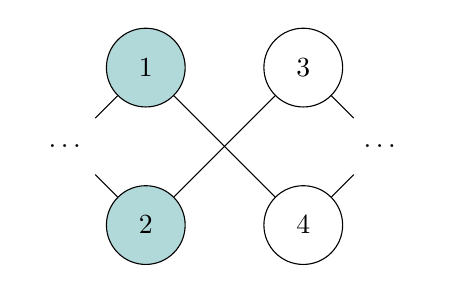
\begin{tikzpicture}[every node/.style={circle, draw, minimum size=1cm}]
			\node[draw=none] (dots1) at (0, 1) {\dots};
			\node[fill=teal!30] (1) at (1, 2) {1};
			\node[fill=teal!30] (2) at (1, 0) {2};
			\node (3) at (3, 2) {3};
			\node (4) at (3, 0) {4};
			\node[draw=none] (dots2) at (4, 1) {\dots};

			\draw (1) -- (4);
			\draw (2) -- (3);

			\draw (1) -- (dots1);
			\draw (2) -- (dots1);
			\draw (3) -- (dots2);
			\draw (4) -- (dots2);
		\end{tikzpicture}
		\caption{Separator in non-planar graph}
	\end{subfigure}
	\hfill
	\begin{subfigure}{0.45\linewidth}
		\centering
		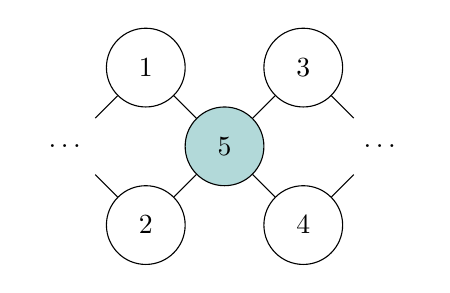
\begin{tikzpicture}[every node/.style={circle, draw, minimum size=1cm}]
			\node[draw=none] (dots1) at (0, 1) {\dots};
			\node (1) at (1, 2) {1};
			\node (2) at (1, 0) {2};
			\node (3) at (3, 2) {3};
			\node (4) at (3, 0) {4};
			\node[fill=teal!30] (5) at (2, 1) {5};
			\node[draw=none] (dots2) at (4, 1) {\dots};

			\draw (1) -- (5);
			\draw (2) -- (5);
			\draw (3) -- (5);
			\draw (4) -- (5);

			\draw (1) -- (dots1);
			\draw (2) -- (dots1);
			\draw (3) -- (dots2);
			\draw (4) -- (dots2);
		\end{tikzpicture}
		\caption{Better separator in planarized graph}
	\end{subfigure}
	\caption{Example of a separator, where a better separator can be found in the planarized graph.}
	\label{fig:planarization_reduces_separator}
\end{figure}

\begin{figure}[tbhp]
	\centering
	\begin{subfigure}{0.45\linewidth}
		\centering
		\begin{tikzpicture}[every node/.style={circle, draw, minimum size=1cm, node distance=1.5cm}]
			\node[fill=teal!30] (1) {1};
			\node[below right=of 1, fill=teal!30] (3) {3};
			\node[left=3cm of 3] (2) {2};
			\node[below left=of 3] (4) {4};

			\draw (1) -- (4);
			\draw (1) -- (2) -- (3);

			\node[right=of 1, draw=none] (dots1) {\dots};
			\node[right=of 4, draw=none] (dots4) {\dots};
			\draw (1) -- (dots1);
			\draw (4) -- (dots4);
			\draw (3) -- (dots4);
			\draw (3) -- (dots1);

			\draw[dashed] (-1, 1) -- (-1, -4.5);
		\end{tikzpicture}
		\caption{Separator in non-planar graph\newline}
	\end{subfigure}
	\hfill
	\begin{subfigure}{0.45\linewidth}
		\centering
		\begin{tikzpicture}[every node/.style={circle, draw, minimum size=1cm, node distance=1.5cm}]
			\node[fill=teal!30] (1) {1};
			\node[below right=of 1, fill=teal!30] (3) {3};
			\node[left=3cm of 3, fill=teal!5] (2) {2};
			\node[below left=of 3, fill=teal!5] (4) {4};
			\node[below= 0.75 of 1, fill=teal!5] (5) {5};

			\draw (1) -- (5);
			\draw (4) -- (5);
			\draw (5) -- (3);
			\draw (1) -- (2) -- (5);

			\node[right=of 1, draw=none] (dots1) {\dots};
			\node[right=of 4, draw=none] (dots4) {\dots};
			\draw (1) -- (dots1);
			\draw (4) -- (dots4);
			\draw (3) -- (dots4);
			\draw (3) -- (dots1);

			\draw[dashed] (-1, 1) -- (-1, -4.5);
		\end{tikzpicture}
		\caption{The separator of the original graph is not a separator in the planarized graph.}
	\end{subfigure}
	\caption{Example where the separator of the original graph is not a separator in the planarized graph.}
	\label{fig:planarization_increases_separator}
\end{figure}



\begin{figure}[tbhp]
	\centering
	\includegraphics[width=0.8\linewidth]{graphics/karlsruhe_top_level_sep_extended_to_planar_wide.png}
	\caption{Visualization of a potential top-level separator for the road network of Karlsruhe.
		Vertices colored teal represent the separator nodes identified within the original, non-planar graph representation.
		Orange vertices (two almost overlapping ones) indicate the additional nodes required to establish a valid separator for the planarized version of the Karlsruhe road network.
		The single teal vertex located on the right side of the figure corresponds to a highway intersection.
		Although seemingly isolated in this view, its inclusion in the separator is necessary.}
	\label{fig:karlsruhe_planar_vs_non_planar}
\end{figure}

These findings highlight that the near-planar structure of road networks has
minimal impact on separator size, suggesting that such networks can typically
be analyzed as planar graphs.







\section{Hierachy}
\label{sec:hierarchy}






\section{Distance and Hop Distribution}
\label{sec:distance_hop_distribution}



\begin{figure}
	\begin{subfigure}{0.45\linewidth}
		\centering
		% \includegraphics[width=\linewidth]{graphics/europe_dist.png}
		\caption{...}
		\label{fig:distance_distribution}
	\end{subfigure}
	\hfill
	\begin{subfigure}{0.45\linewidth}
		\centering
		% \includegraphics[width=\linewidth]{graphics/europe_hops.png}
		\caption{...}
		\label{fig:hop_distribution}
	\end{subfigure}
	\caption{...}
	\label{fig:distance_hop_distribution}
\end{figure}


